\SACCMD{map}
\label{cmd:map}

\SACTitle{概要}
利用SAC内存中的所有数据文件生成一个包含台站/事件符号、地形以及台站名的
GMT地图,也可以在命令行上指定一个事件文件。每个
地震事件符号可以根据震级、残差等确定其大小。这个命令会产生一个ps文件,
并将该文件在屏幕上显示,同时产生一个绘制该图的shell脚本。

\SACTitle{语法}
MAP\quad [ MERcator | EQuidistant | AZimuthal\_equidistant | ROBinson ] [ WEST minlon ] [ EAST maxlon ] [ NORTH maxlat ] [ SOUTH minlat ] [ MAGnitude | REsidual | RMean\_residual ] [ EVentfile filename ] [ TOPOgraphy ] [ STANames ] [MAPSCALE on | off ] [ PLOTSTATIONS on | off ] [ PLOTEVENTS on | off ] [ PLOTLEGEND on | off ] [ LEGENDXY x y ] [ FILE output-file ]

\SACTitle{输入}
SAC中可以使用的投影方式包括:
\begin{itemize}
\item MERCATOR:	投影方式为Mercator投影。
\item EQUIDISTANT: 投影方式为等间距圆柱投影,经纬度为线性。
\item ROBINSON: 投影方式为Robinson投影,适用于世界地图。
\item LAMBERT: 适用于东西范围较大的区域。
\item UTM:通用横向Mercator(尚未实现)。
\end{itemize}

下面的选项允许用户指定地图的区域,其默认使用台站以及事件经纬度的最小最大值(如果真是如此,这样的缺省值并不合适,因为那样意味着某些台站或事件将位于地图的边界处,但是实际上地图范围给的还是不错的):
\begin{itemize}
\item WEST :  地图的最小经度 
\item EAST : 地图的最大经度 
\item NORTH : 地图的最大纬度 
\item SOUTH : 地图的最小纬度 
\item AUTOLIMITS:  自动决定地图的区域 [缺省值] 
\end{itemize}
  
下面的选项允许用户向地图中添加位置和注释:
\begin{itemize}
\item STANames on | off :  在地图上绘制台站名[默认为off]
\item MAPSCALE on | off :  在地图上绘制地图比例尺[默认为off]
\item PLOTSTATIONS on | off : 绘制地震图给出的全部台站[默认为on]
\item PLOTEVENTS on | off : 绘制eventfile和/或地震图给出的全部事件[默认为on]
\end{itemize}

下面的选项允许用户根据不同的值给出不同地震事件符号的大小。默认值是所有符号大小一样:
\begin{itemize}
\item MAGnitude : user0定义地震震级,user0越大,则事件符号越大。
\item REsidual : user0定义残差。根据user0的绝对值定义事件符号的大小。正值为(+) 负值为(-).
\item RMean\_residual : 与residual相同,除了将所有残差去除均值之外
\item PLTLEGEND on | off : 绘制地震震级以及残差的图例[默认为on] 
\item LEGENDXY x y : 绘制图例的绝对位置,默认为[1,1]。位置是相对于页面的左下角,其单位为inch。 这是一个与地震震级和残差有关的图例。
\item EVENTFILE : 指定一个自由格式的ASCII文本文件,其包含了额外的事件数据,文件的每一行包含单个事件的数据。每行的头两列必须包含纬度和经度(单位为度)。第三列可以包含符号大小信息(比如震级、深度、走时残差等)。
\item TOPOgraphy on | off : 设置TOPO为开允许用户向地图中添加地形和海洋深度。这个命令读取GMT中grdraster.info的第一个地形文件,当然地形文件中必须要有该区域的数据。地形彩色图使用\$SACAUX/ctables/gmt.cpt。网格文件被写入当前目录
\item FILE : 默认的输出文件名为gmt.ps,你可以通过FILE选项指定文件名
\end{itemize}
可以用SAC的TITLE命令指定其标题

\SACTitle{缺省值}
   MAP MERCATOR TOPO off STAN off FILE gmt.ps PLOTSTATIONS on PLOTEVENTS on

\SACTitle{例子}
利用SAC提供的一些数据作为例子:
\begin{SACCode}
SAC> r /opt/sac/aux/datagen/regional/*.z
SAC> map stan on 
Using Default Postscript Viewer
	gs -sDEVICE=x11 -q -dNOPROMPT -dTTYPAUSE 
	Set an alternative through the SACPSVIEWER environment variable
	Press any key to continue
\end{SACCode}
绘制出的地图如图\ref{fig:map}所示,整个地图的边界控制的还算不错,还算比较美观,
三角形代表台站位置,圆形代表地震位置,大小也控制的不错。生成这个图的同时,还有
一个可以用于生成该地图的shell脚本。
\begin{SACCode}
#!/bin/csh -f

# Set the output file
set psfile = "./gmt.ps"

# Start the Postscript file 
psbasemap -JM6.5i -R-120.572/-110.404/33.754/41.380 \
-Ba3.000f3.000/a2.000f2.000NEWS:."": -X0.75i -Y1.0i -P -K > $psfile 

# Add the Coastline and National Boundaries
pscoast -K -O -J -R -B -N1 -N2 -W -Dl -A78 -G250/250/200  >> $psfile 

# Add station location labels.  
# Input are longitude, latitude, and name.
pstext -K -O -D0.10i/0.10i -J  -R -S0.25/255 -G0/0/0 <<EOF >> $psfile 
-115.239 40.745  10 0 0 BL  ELK      
-112.822 37.017  10 0 0 BL  KNB      
-116.411 34.390  10 0 0 BL  LAC      
-118.154 38.432  10 0 0 BL  MNV      
EOF

# Add station locations.  
# Input are longitude latitude.
psxy -K -O -J -R -St0.25i -G0/0/0 <<EOF >> $psfile 
-115.239 40.745 
-112.822 37.017 
-116.411 34.390 
-118.154 38.432 
EOF

# Add event locations.
# Input are longitude latitude.
psxy -O -K -J -R -W10/0/0/0  -Sc0.25i  <<EOF >> $psfile 
-118.123 37.852 
EOF

# End the Postscript File
psxy -R -J -O /dev/null >> $psfile 
\end{SACCode}

\begin{figure}[h]
\centering
\caption{map例子示意图}
\label{fig:map}
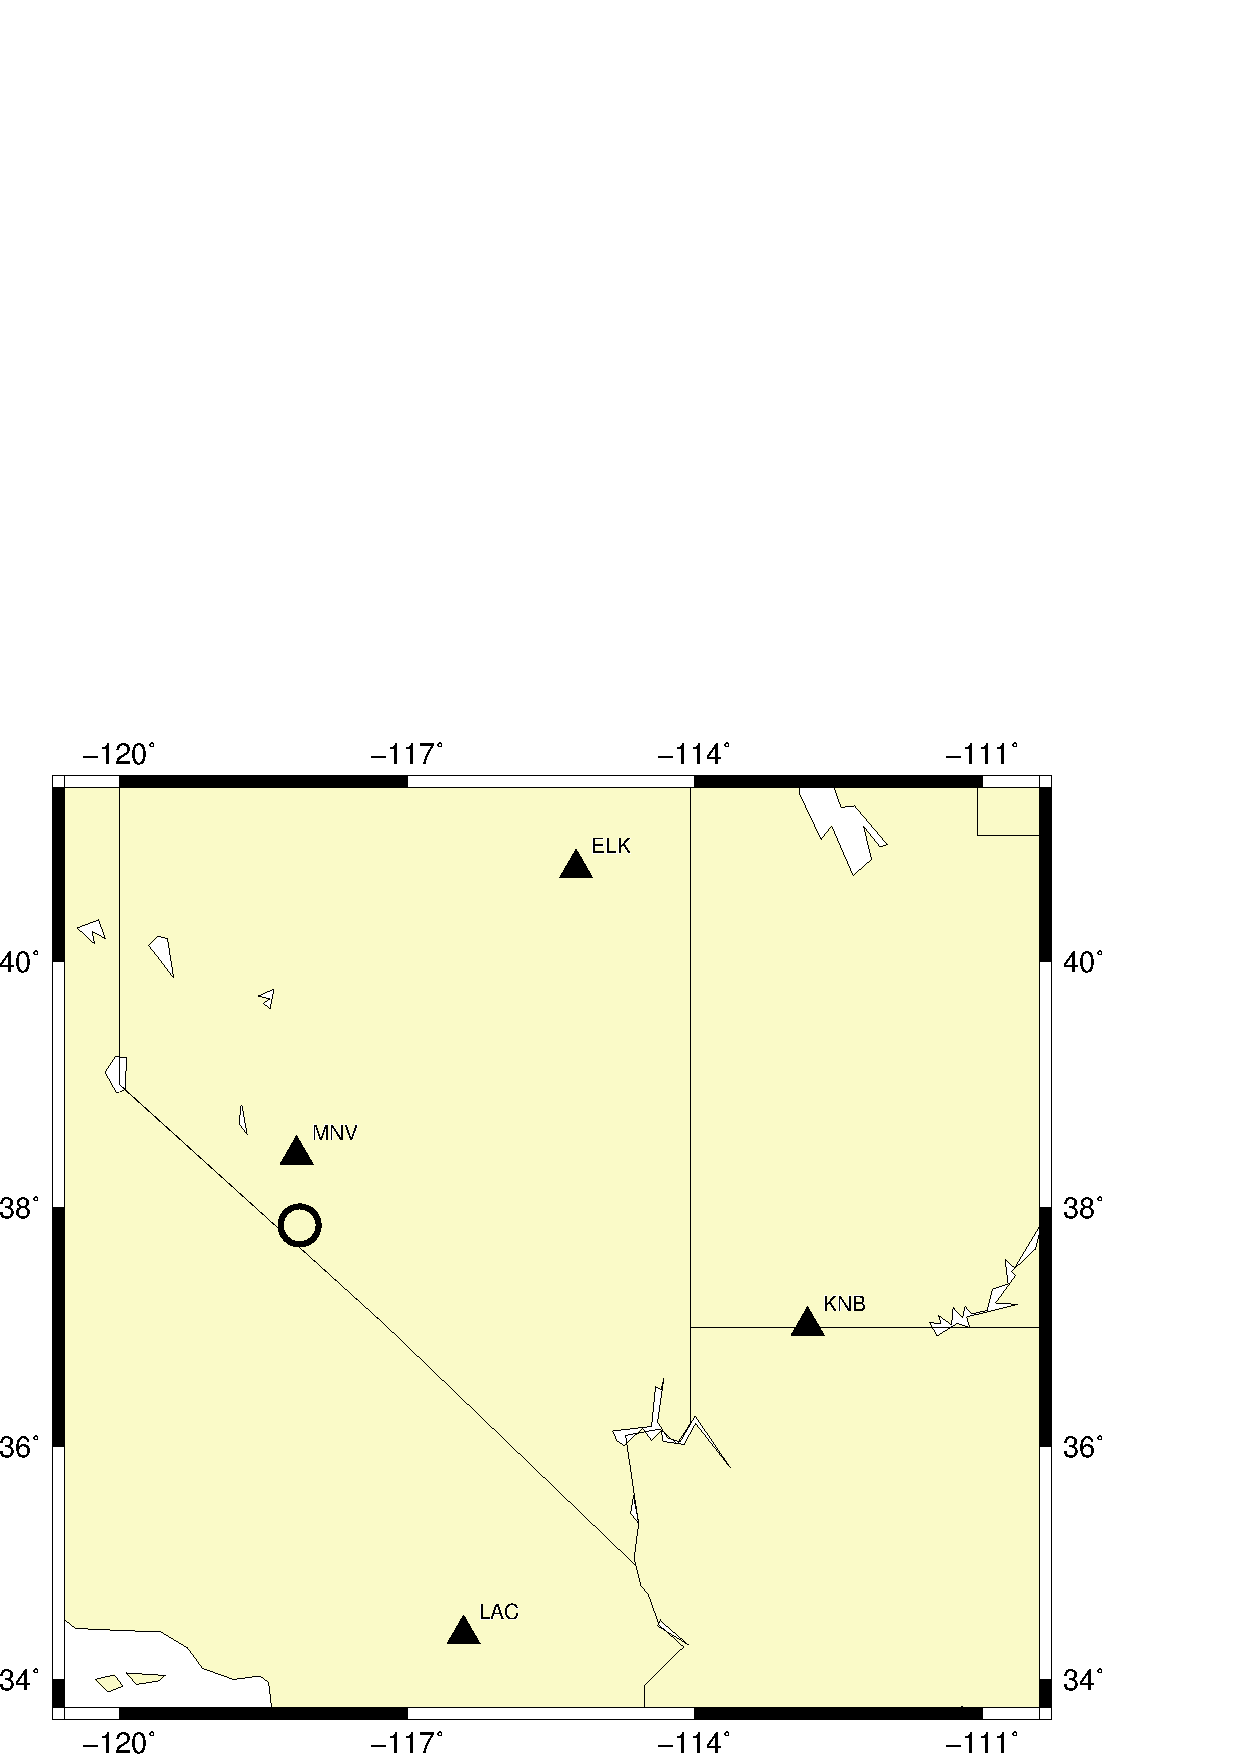
\includegraphics[width=10cm]{map}
\end{figure}

\SACTitle{头段数据}
台站纬度(stla)以及经度(stlo)必须在头段中被定义。如果事件纬度(evla)以及经度(evlo)被定义则其会被包含在地图中。如果这个命令在执行BBFK之后执行,MAP将沿着反方位角方向绘制大圆弧路径。
这个版本的MAP是基于4.0版本的Generic Mapping Tools,要执行这个命令,你需要将GMT4.0安装在你的机器上并保证可执行文件位于路径中。

每个MAP命令的结果将写入当前目录下一个称为gmt.csh的脚本中。用户可以修改这个文件以利用更多SAC未利用的选项。默认单位是inch,当然可以在脚本中修改。

在使用pscoast绘制海岸线时,SAC采用了-Dl选项,其中l代表低精度的海岸线数据。用户
可以在脚本中修改使用更高精度的海岸线数据。

该脚本采用的shell是csh,其很容易改成bash脚本。

MAP命令的结果将自动被显示。用于显示的默认程序是gs(ghostscript)。用户可以通过设置环境变量SACPSVIEWER选择其他显示工具。\\
在csh下可以这样设置:
\begin{SACCode}
setenv SACPSVIEWER "gs -sDEVICE=x11 -q -dNOPROMPT -dTTYPAUSE"
\end{SACCode}
在bash下可以这样设置:
\begin{SACCode}
export SACPSVIEWER="gs -sDEVICE=x11 -q -dNOPROMPT -dTTYPAUSE"
\end{SACCode}
